% ============================================================================
% APPENDIX: GAN Hyperparameter Optimization — Surrogate Landscapes
%           and Non-Linearity Analysis
% ============================================================================
% Add this as a new appendix section (e.g., Appendix J) after the existing
% appendices (A through I).
%
% Figures required (all in figures/):
%   appendix_gan_landscapes.png      — 2x2 gen/disc landscapes
%   appendix_gan_nonlinearity.png    — 2x3 additivity test heatmaps
% ============================================================================

\section*{J. GAN Surrogate Landscapes and Interaction Analysis}

\subsection*{J.1 Child Hyperparameter Landscapes}

Figure~\ref{fig:app_gan_landscapes} shows the FID landscape for each
child sub-problem in both surrogate tasks.

\textbf{Standard task} (top row).
The generator landscape (a) is smooth and dominated by learning rate:
FID degrades sharply for $\text{LR}_\text{gen} \geq 5 \times 10^{-3}$,
while weight decay has a comparatively mild effect.
The discriminator landscape (b) is more complex, with a narrow basin of
good configurations at intermediate learning rates
($2 \times 10^{-4}$--$10^{-3}$) and low-to-moderate dropout ($0.0$--$0.3$).
High learning rates or high dropout both cause catastrophic FID increases.

\textbf{SpectralNorm task} (bottom row).
The generator landscape (c) retains the same qualitative structure as in
the standard task---low learning rates are preferred---consistent with
the shared generator architecture.
The discriminator landscape (d), however, shifts noticeably:
Spectral Normalization stabilizes training, broadening the region of
acceptable configurations and reducing the dropout sensitivity.
This landscape shift is precisely the change that the modularity
experiment exploits: the generator child transfers directly, while
the discriminator child must be re-learned.

\begin{figure}[h]
\centering
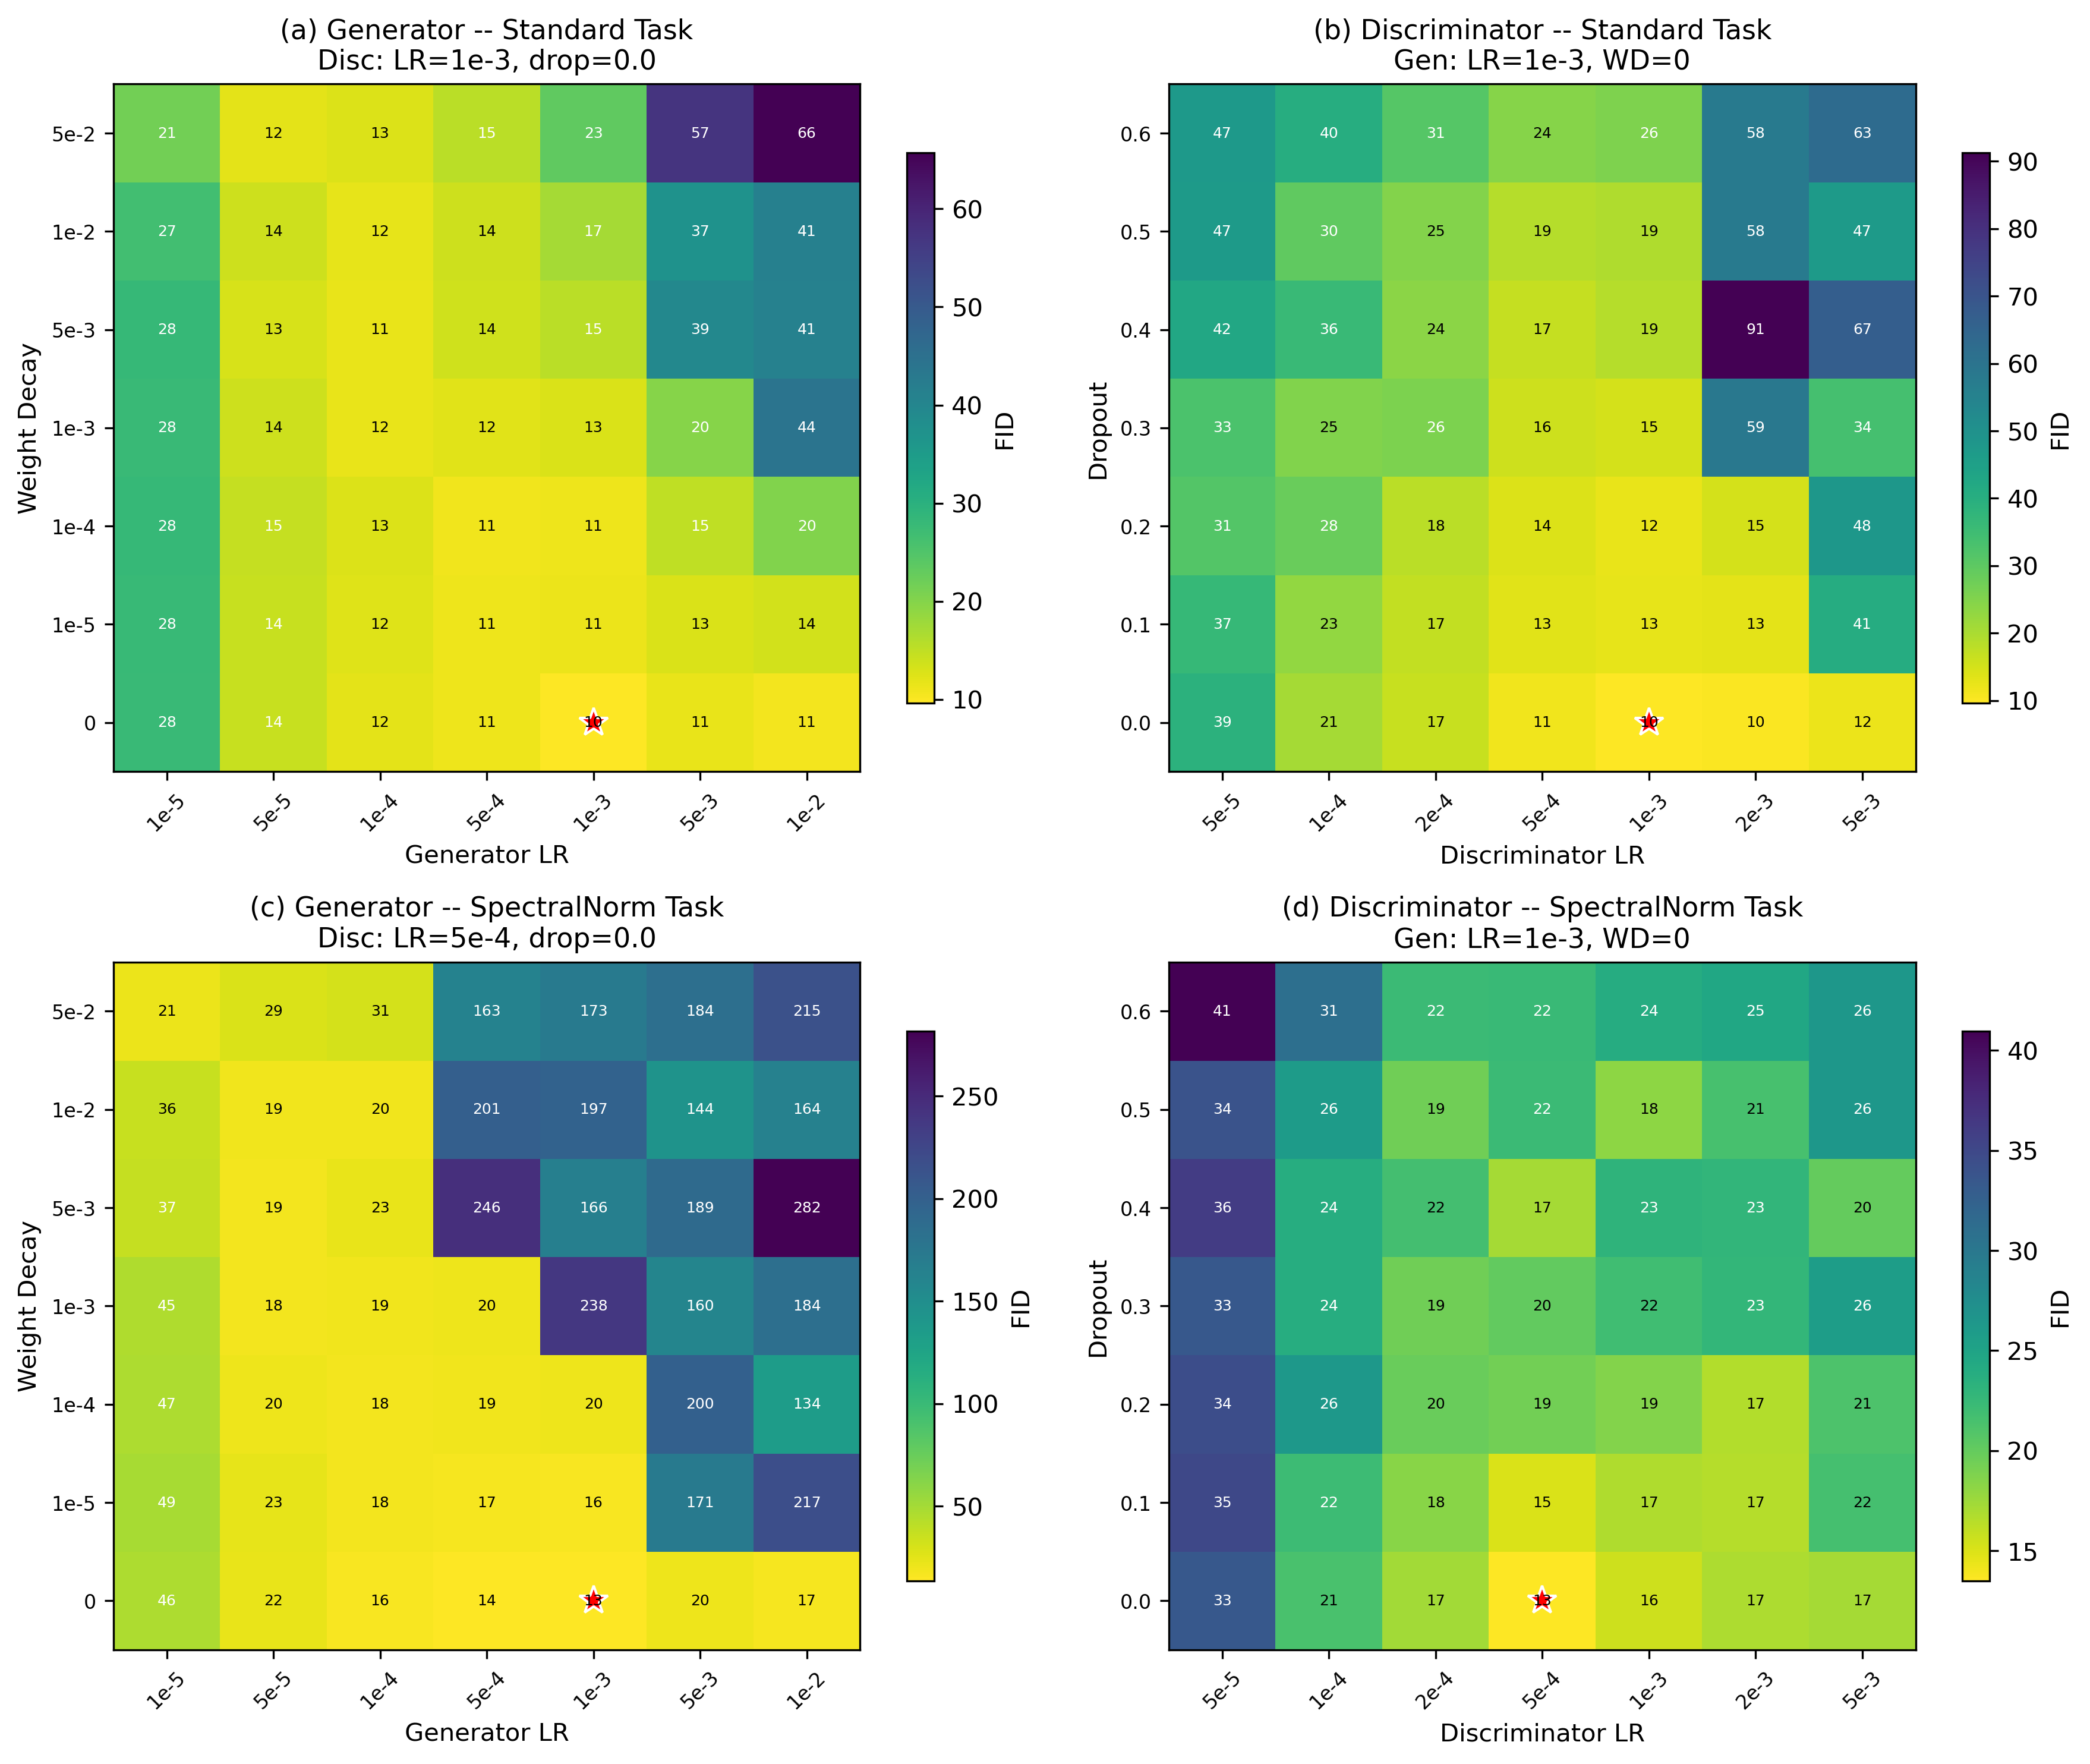
\includegraphics[width=\textwidth]{figures/appendix_gan_landscapes.png}
\caption{Child hyperparameter landscapes for the GAN surrogate.
\textbf{Top:} Standard task (BatchNorm discriminator).
\textbf{Bottom:} SpectralNorm task.
Each heatmap shows FID (lower = better) as a function of the child's
two hyperparameters, with the other child fixed at its task-specific optimum.
Red stars mark the global optimum.}
\label{fig:app_gan_landscapes}
\end{figure}


\subsection*{J.2 Non-Linear Interaction Between Generator and Discriminator}

BIF assumes a quasi-linear additive interaction between children
(Section~3): $F(x) \approx f_{\text{gen}}(x_{\text{gen}}) + f_{\text{disc}}(x_{\text{disc}}) + c$.
To quantify how well this assumption holds for the GAN surrogate,
we perform an ANOVA-style variance decomposition.
Let $Y_{ij}$ denote the neg-FID for generator configuration $i$ and
discriminator configuration $j$.
The additive reconstruction is
$\hat{Y}_{ij} = \bar{Y}_{i \cdot} + \bar{Y}_{\cdot j} - \bar{Y}_{\cdot \cdot}$,
where $\bar{Y}_{i \cdot}$, $\bar{Y}_{\cdot j}$, and $\bar{Y}_{\cdot \cdot}$
are the row, column, and grand means respectively.
The residual $R_{ij} = Y_{ij} - \hat{Y}_{ij}$ captures the non-additive
(interaction) component.

Table~\ref{tab:app_nonlinearity} summarizes the decomposition.
For the \textbf{standard task}, the additive model explains only
$45.5\%$ of total variance ($R^2 = 0.455$), with $54.5\%$ attributable to
gen-disc interaction.
This substantial non-linearity means that the optimal generator
configuration depends on which discriminator is used, and vice versa
--- a challenging scenario for any additive-prior method.
For the \textbf{SpectralNorm task}, additivity improves to $R^2 = 0.804$,
with only $19.6\%$ interaction variance, likely because Spectral
Normalization reduces the discriminator's sensitivity to generator
choices.

\begin{table}[h]
\centering
\small
\begin{tabular}{lccc}
\toprule
Task & Additive $R^2$ & Interaction (\% of var) \\
\midrule
Standard (BatchNorm)  & 0.455 & 54.5\% \\
SpectralNorm          & 0.804 & 19.6\% \\
\bottomrule
\end{tabular}
\caption{Variance decomposition of the GAN surrogates.
The additive model $\hat{Y}_{ij} = \bar{Y}_{i\cdot} + \bar{Y}_{\cdot j} - \bar{Y}_{\cdot\cdot}$
is compared to the true neg-FID table.
The standard task exhibits strong non-linear gen-disc interaction
($54.5\%$ of variance), while SpectralNorm reduces this to $19.6\%$.}
\label{tab:app_nonlinearity}
\end{table}

Figure~\ref{fig:app_nonlinearity} visualizes this decomposition.
The residual heatmaps (c, f) reveal structured interaction patterns:
in the standard task, specific gen-disc combinations produce
FID values far from what either marginal would predict,
particularly at high generator learning rates.
Despite this violation of additivity, BIF's performance
remains competitive (Table~1), demonstrating the robustness
noted in Appendix~G.

\begin{figure}[h]
\centering
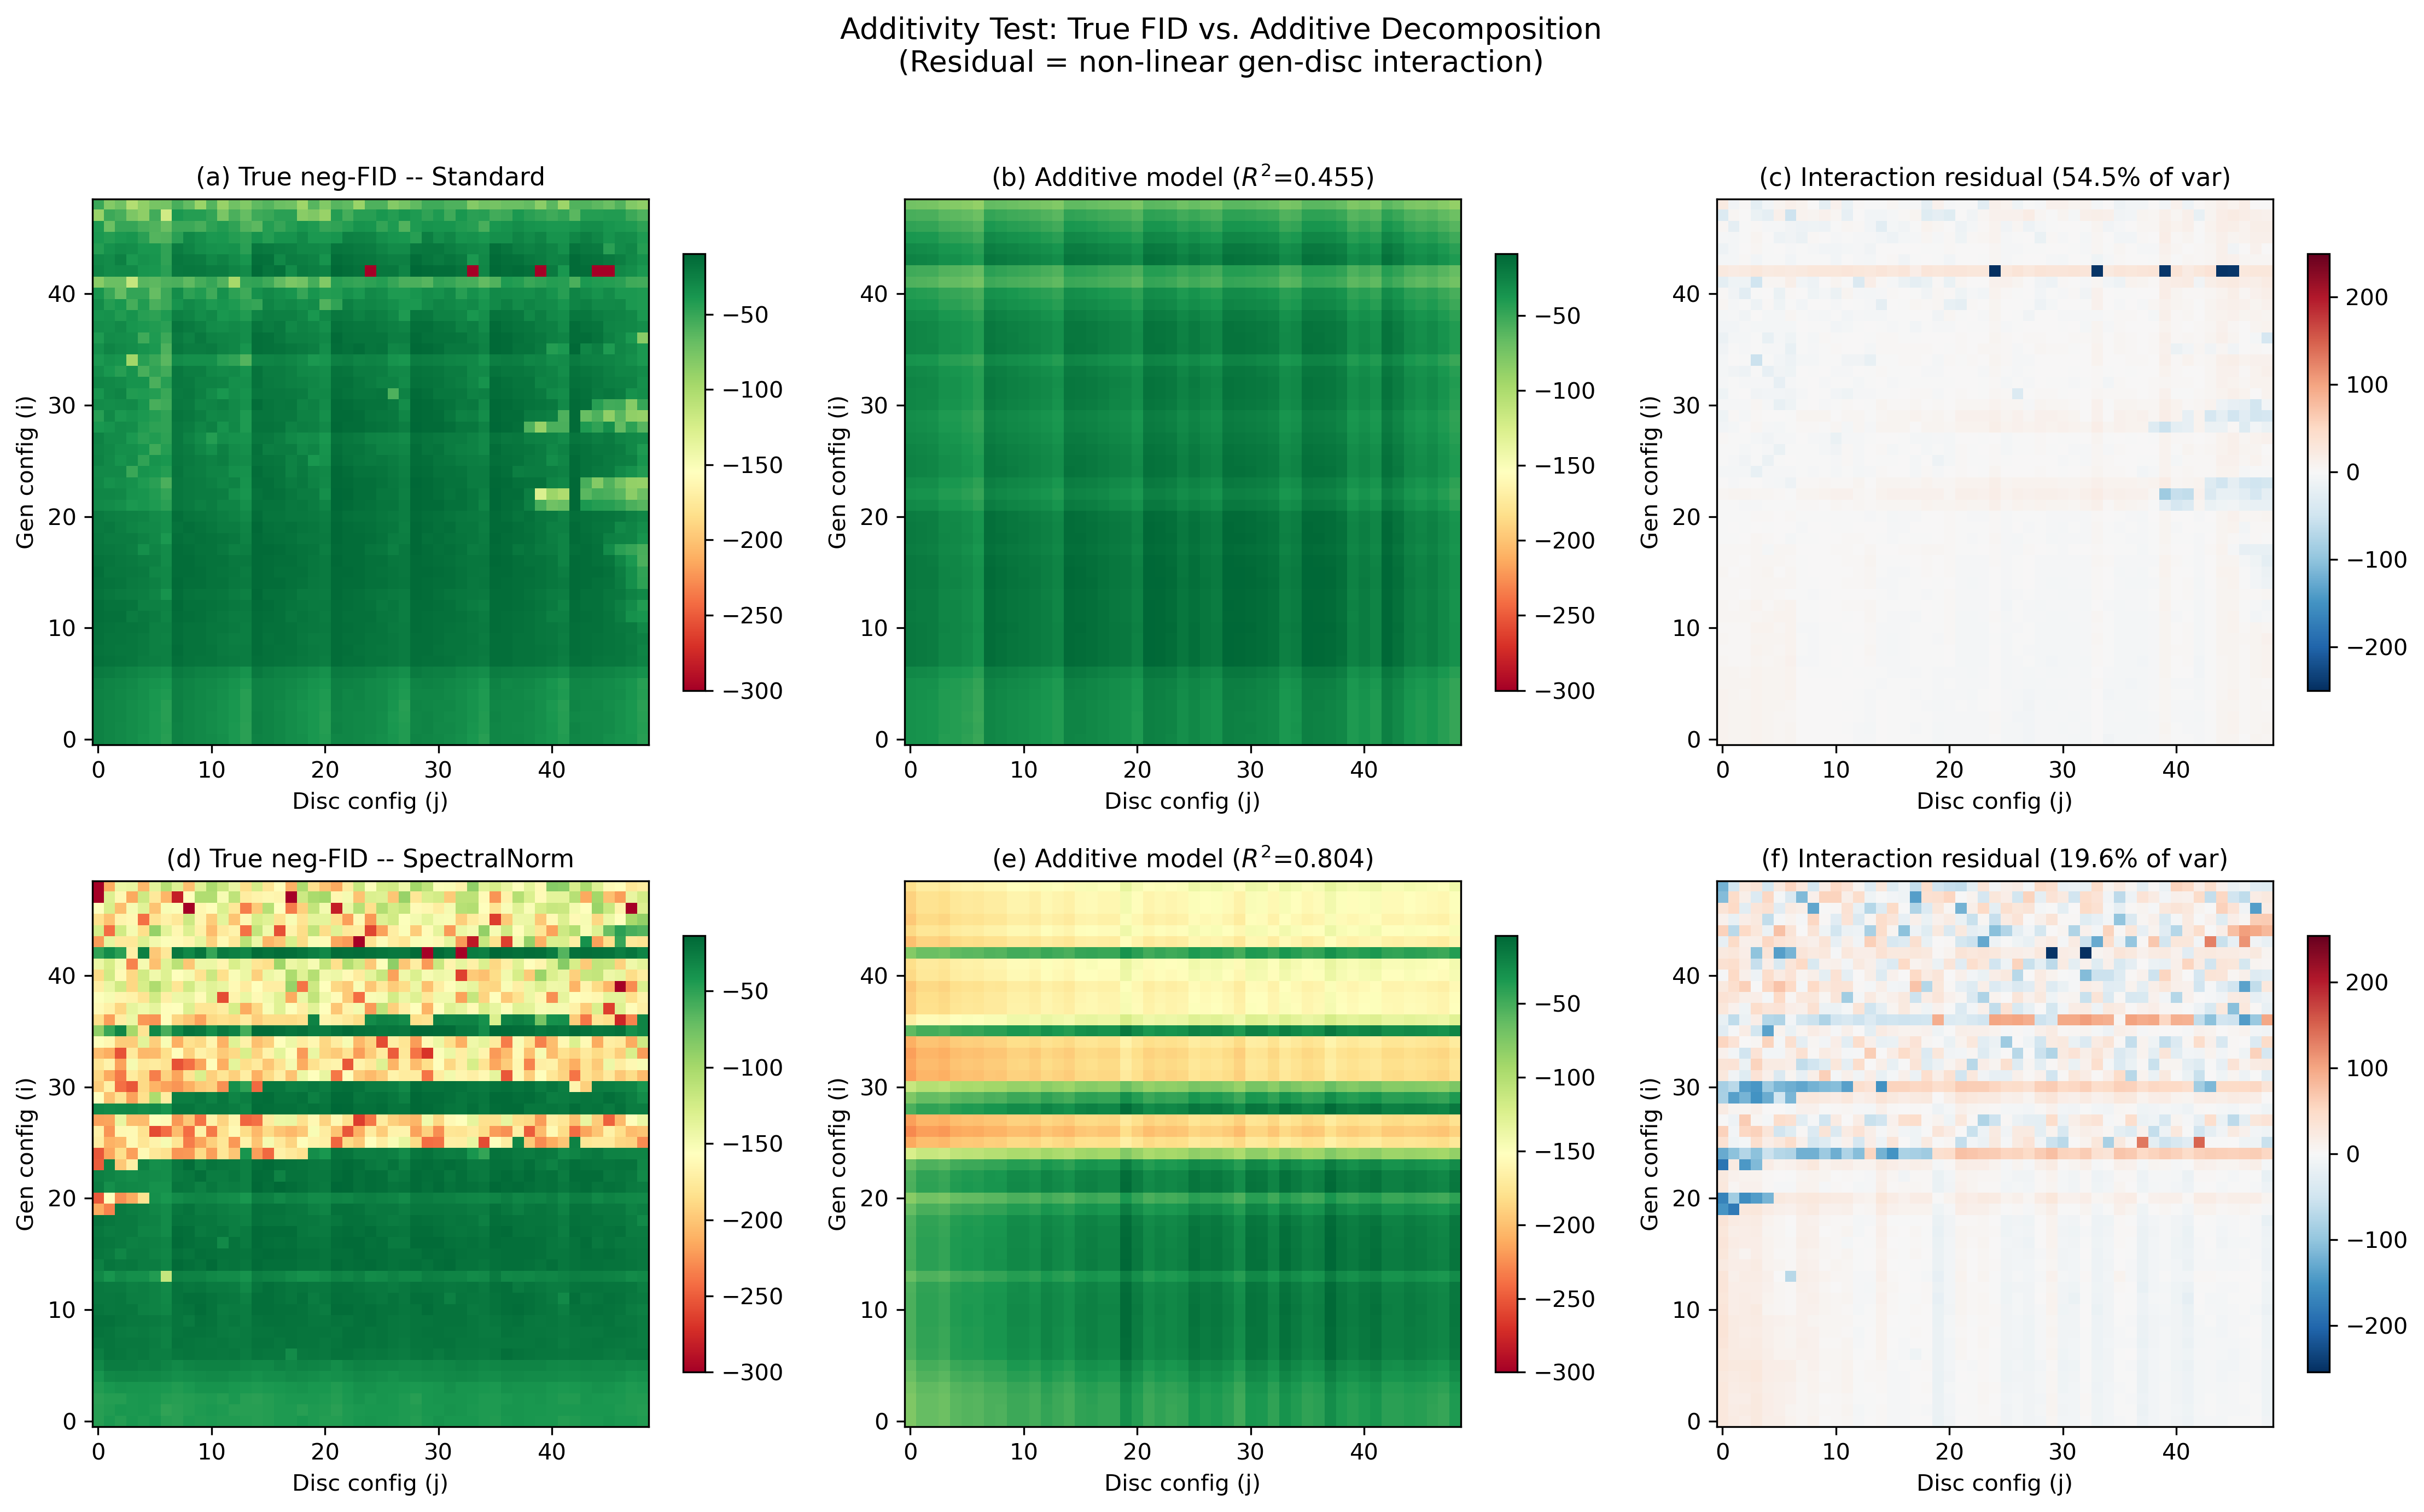
\includegraphics[width=\textwidth]{figures/appendix_gan_nonlinearity.png}
\caption{Additivity test for the GAN surrogates.
\textbf{Left:} True neg-FID landscape (49 gen configs $\times$ 49 disc configs).
\textbf{Center:} Additive reconstruction from marginal means.
\textbf{Right:} Residual (interaction component), plotted on a
diverging colormap (red/blue = positive/negative deviation from additivity).
\textbf{Top row:} Standard task ($R^2 = 0.455$, $54.5\%$ interaction).
\textbf{Bottom row:} SpectralNorm task ($R^2 = 0.804$, $19.6\%$ interaction).}
\label{fig:app_nonlinearity}
\end{figure}
